% !TeX root = ../main.tex
% Add the above to each chapter to make compiling the PDF easier in some editors.


\chapter{Approach}\label{chapter:approach}

%%%%%%%%%%%%%%%
%%% Dataset
%%%%%%%%%%%%%%%
\section{Ground Truth Dataset}\label{dataset}
The basis for our work is a dataset of 100,000 synthetic tumors of resolution $128^3$ that were generated by
randomly sampling patient-specific parameters from the subsequent ranges:
\begin{gather*}
    D_w \in [0.0002 \frac{cm^2}{d}, 0.015 \frac{cm^2}{d}] \\%= [7.3 \frac{mm^^2}{yr}, 547.5 \frac{mm^^2}{yr}], 
    \rho \in [0.002 \frac{1}{d} , 0.2 \frac{1}{d}], \\ %= [0.73 \frac{1}{yr}, 73 \frac{1}{yr}] ,
    T \in [50d, 1500d], \\
    x \in [0.15,0.7], y \in [0.2, 0.8], z \in [0.15, 0.7]
\end{gather*}

To further improve realism and overall quality of the data, tumors that would likely not occur in a clinical setting due to their size have been removed based on minimal and maximal size thresholds, as can be seen in \parencite{Steinbauer2020}. The used thresholds are derived from the BraTS dataset as defined in \parencite{MenzeMultiModalApproach}.\\
Due to the time and therefore also runtime limitations of our project, only a random subset of 50,000 tumors has been used for all experiments throughout this project, which will be referred to as $S$.\\
For testing the quality of our following experiments, we used a Dataset of 63 MRI scans of patients diagnosed with glioblastoma provided by the MRI TUM Klinikum Rechts der Isar. Based on these scans, we generated a Dataset $P$ containing binary segmentations representing the scans' FLAIR ($P^{FLAIR}$) and T1Gd ($P^{T1Gd}$) modalities.


%%%%%%%%%%%%%%%
%%% Pipeline
%%%%%%%%%%%%%%%
\section{Learn-Morph-Infer Pipeline}\label{pipeline}
The main goal of this paper is to propose an alternative step within the learn-morph-infer pipeline presented in \parencite{LearnMorphInfer} that ideally leads to more deterministic and reliable results.
Thus, it is indispensable to first understand the original pipeline, which consists of four main steps:\\
% include image here
First, a patient MRI scan of a tumor observation $Y = \{y^{T1Gd}, y^{FLAIR}\}$ is registered to the atlas brain anatomy, yielding a transformation matrix $M$.
Afterwards, $M$ is used to morph $Y$ into the atlas space resulting in $Y_{atlas}$.
Subsequently, a neural network, that was pretrained on the dataset seen in \autoref{dataset} to learn the function $Y_{atlas} \mapsto \theta_c$, infers a set $\theta_c$ of patient-specific parameters, which is then used as an input for a tumor solver in step 3 to generate a patient specific tumor simulation in the atlas space. 
As a last step, utilizing the inverse of $M$, the atlas simulation is morphed back to the patient brain anatomy to obtain the final patient-specific simulation \parencite{LearnMorphInfer}.

\begin{figure}[htbp]
  \centering
  \includesvg[width=350pt]{figures/pipeline_base}
  \caption{A sketch showcasing the learn-morph-infer pipeline. A patient MRI scan is registered to the atlas space (1). Then, a neural network infers patient-specific parameters from the morphed scans (2), which serve as input for a tumor solver that yields a tumor simulation in the atlas space (3). Finally, the output is morphed back to the patient brain anatomy to obtain the patient-specific simulation (4).}
\end{figure}

Applications of this pipeline, e.g.\parencite{Scibilia2021}, are able to produce fairly accurate results (average Dice scores of roughly 0.9) in the order of seconds. However, neural networks always come with the drawback of being unpredictable for unseen data, which introduces a potential risk.\\\\
In the following, we propose a deterministic approach to overcome this limitation. Instead of using a neural network to infer $\theta_c$, which can then be passed to a tumor solver, we suggest making a simple query to a database of synthetic tumors and returning the closest match as a result. The rest of the pipeline, namely the forward and reverse registration, remains unchanged. The following sections will discuss different ways to implement this surrogate.

\begin{figure}[htbp]
  \centering
  \includesvg[width=350pt]{figures/pipeline_db_query}
  \caption{A sketch showcasing the proposed adaption to the learn-morph-infer pipeline. A patient MRI scan is registered to the atlas space (1). Subsequently, a query to a database of tumors is executed to the closest match for the morphed scans (2). This best match tumor is then morphed back to patient brain anatomy to obtain the patient-specific simulation. (3)}\label{fig_query_pipeline}
\end{figure}

%%%%%%%%%%%%%%%
%%% Baseline
%%%%%%%%%%%%%%%
\FloatBarrier
\section{Baseline}
The most basic way to implement the change to the learn-morph-infer pipeline proposed in \autoref{pipeline} and visualized in \autoref{fig_query_pipeline} is by naively looping over the dataset and performing a pair-wise comparison between input and database tumors. In order to achieve a meaningful comparison, a fitting metric is required.
For 3 dimensional binary data, the Dice score is a common option \todo{SRC} and therefore used as the primary metric. In order to also allow direct comparison with vectors in the following sections, we also use the L2 metric.
Moreover, the suggested step requires 2 separate queries - one for each segmentation - and might therefore produce 2 different best matches. Hence, the 2 results have to be combined to find a joint best match. For simplicity, we decided to simply add the 2 individual similarity values and choose the highest combined value for Dice and respectively the lowest for L2 as the best match. 
We implemented this basic brute-force loop in a python script to create a ground truth that serves as a reference for later improvements and experiments.
Since the individual comparisons are not dependent on each other, we made a first optimization by parallelizing the loop to shorten its runtime.

\subsection{Downsampling}
Another potential optimization that is still quite close to the baseline is down sampling. Due to the tumors' relatively high resolution of $128^3$, a lot of data has to be loaded and compared. This overhead can be reduced by down sampling the data to lower resolutions. In our case, we tried a down sampling to $64^3$. \todo{maybe add 32} The down sampling process is achieved by applying a spline interpolation or order 0 to the volume. 


%- metric? -> dice better for volume data, using l2 as well since its better for vectors which are later needed for the encoded data\newline
%- groundtruth baseline is a iterative pairwise comparison\newline
%- improvements: parallelize, downsampling

%%%%%%%%%%%%%%%
%%% Autoencoder
%%%%%%%%%%%%%%%
\section{Compression}
Although parallelization and down sampling can help to reduce the time complexity of the database query, the speed of this operation is still limited by the significant memory usage. This restriction also prohibits the use of efficient query frameworks. For instance, the FAISS library is designed for vector sizes in the range of roughly 20 - 2000 \parencite{FAISS}. However, a plain flattening of our 3D volume of $128^3$ exceeds this suggested limit by a factor of more than 1000. Therefore, we decided to experiment with a compression of the data. Since basic compression usually does not preserve similarity relationships \todo{check with paper!},  we decided to examine if an Autoencoder is able to create a problem-specific encoding that might be able to sufficiently preserve similarity relationships between tumors.

\subsection{Autoencoder}\label{autoencoder}
An Autoencoder is a deep learning method that tries to reconstruct the input data after being put through a hidden layer $h$, often also referred to as latent space, that represents an encoding. Therefore, it consists of an encoder function $h=enc(x)$ and a decoder $r = dec(h)$ producing a reconstruction $r$. The goal is to minimize the difference between $x$ and $r$ while restricting the hidden layer to be of a smaller dimension than the input, producing a bottleneck. Ideally, the Autoencoder learns to extract meaningful features from the input data, since it is forced to prioritize which input features are relevant \parencite{Goodfellow-et-al-2016}.
A visualization of this concept for our use case can be found in \autoref{autoencoder_brain}.\\
The core idea is to train the autoencoder to extract meaningful properties of the tumors and then apply the encoder
function to the dataset $S$, yielding an encoded dataset $S_{enc}$.
For each query, we utilize $S_{enc}$ and encode the input tumor using the same encoder, resulting in a data size drop from $128^3$ to the dimension of the latent space per tumor. Since the segmentations $y^{T1Gd}$ and $y^{FLAIR}$ differ in their properties, two separate autoencoders are needed, leading to consequently two encoded Datasets $S_{enc}^{T1Gd}$ and $S_{enc}^{FLAIR}$.

\begin{figure}[htbp]
  \centering
  \includesvg[width=320pt]{figures/autoencoder_brain}
  \caption{Visualization of the autoencoder usage in our scenario}\label{autoencoder_brain}
\end{figure}

\FloatBarrier
\subsubsection{Neural Network}\label{autoencoder_network}
The base architecture is a convolutional neural network (CNN). In the decoder, we scale down the volume layer-by-layer using strided 3D convolutions (stride=2, kernel size=3) followed by a convolution without stride, while increasing the number of channels. After down scaling the volume, we flatten the features and apply a linear layer to obtain a latent representation. Afterwards, the decoder mirrors this process with strided 3D transposed convolutions.\\
In order to determine a fitting value for the smallest resolution, multiple test runs have been executed, which suggested that a down scaling to a resolution of $16^3$ yields the most reasonable results. This minimal resolution was used throughout all consecutive trainings. 
The final architecture can be seen in \autoref{autoencoder_network}.

\begin{figure}[htbp]
  \centering
  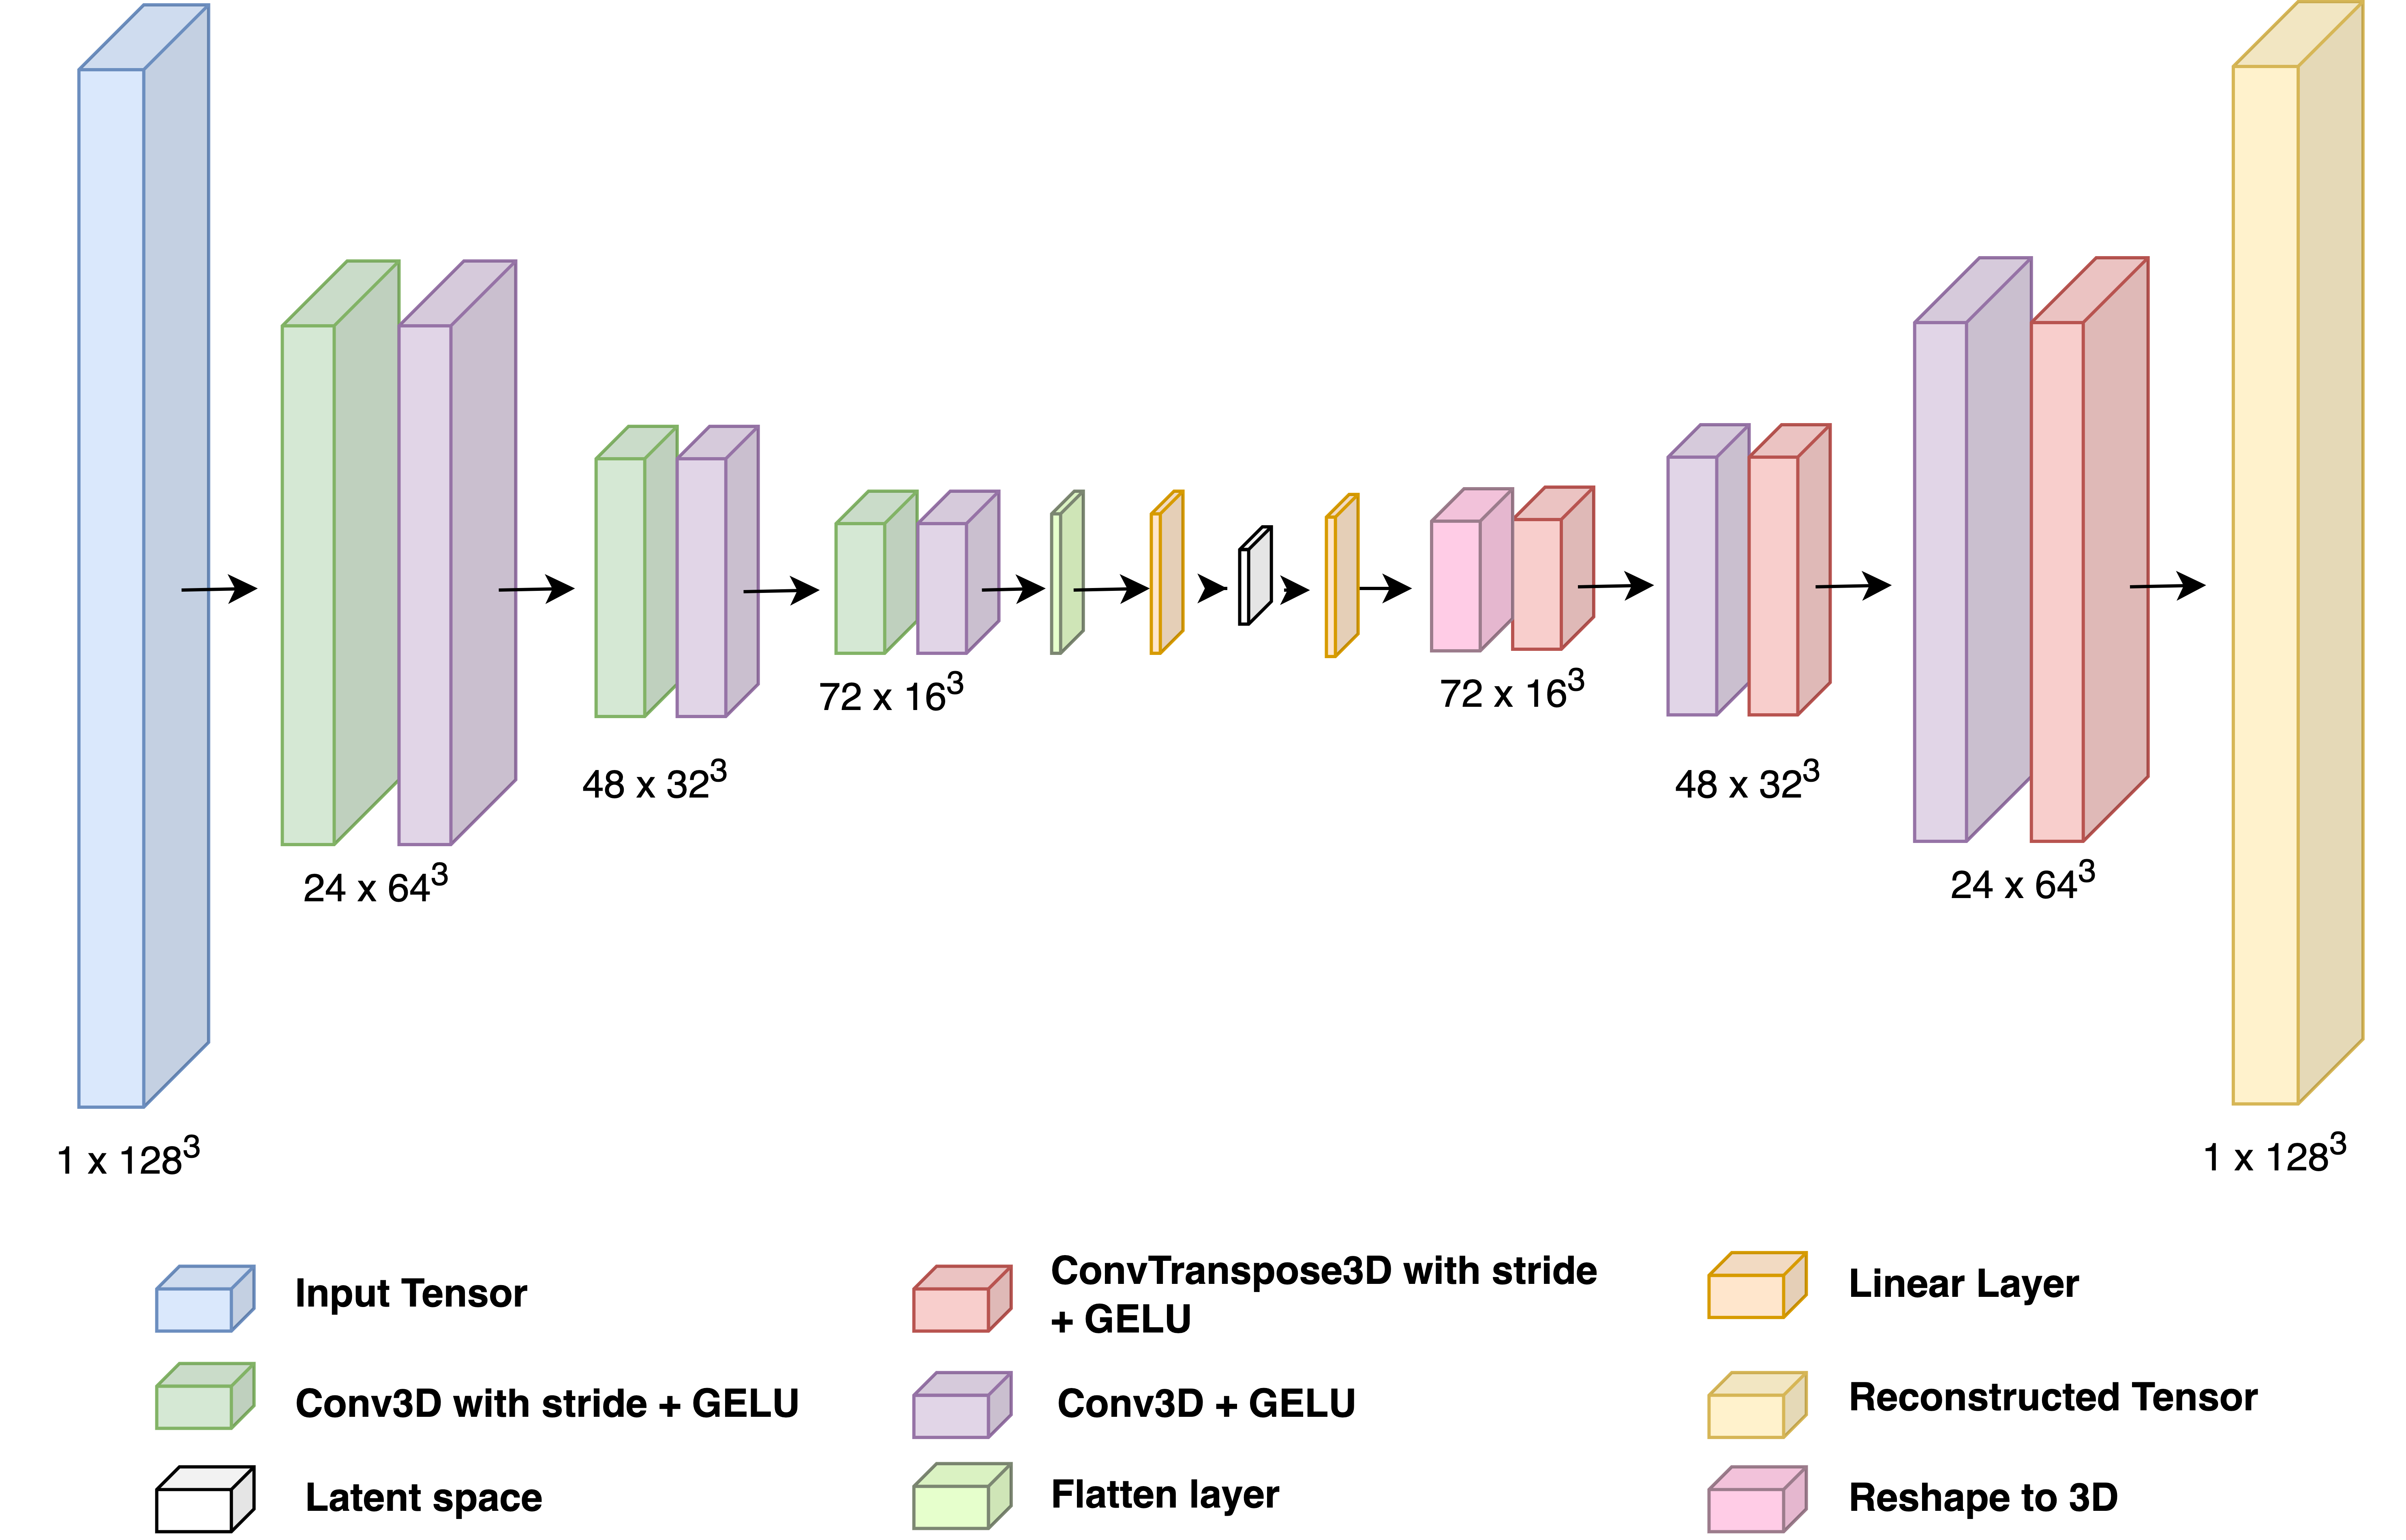
\includegraphics[width=450pt]{figures/autoencoder_network}
  \caption{Autoencoder network showcasing order and type of individual layers}\label{fig_autoencoder_network}
\end{figure}
\FloatBarrier

\subsubsection{Training}\label{autoencoder_training}
The network shown in \autoref{fig_autoencoder_network} was trained for both $y^{T1Gd}$ and $y^{FLAIR}$ as input. Since larger training set sizes showed no significant improvements, we used a relatively small training set of 1500 tumors along with a validation set of size 150.
Experiments suggested a learning rate of $1e^{-5}$ combined with the Adam optimizer. Different losses including Binary Cross Entropy (BCE), Mean Squared Error (MSE) and a variation of Dice losses were tested out of which the default Dice loss produced the best training results.
In terms of batch size, small values improved train quality, leading to a final choice of 2.\todo{Batch size details?}
Another important parameter is the size of the latent space. Motivated by the need of a significant data compression, coupled with the excessive GPU memory usage (> 48 GB) of networks with fully connected layers beyond a latent space size of 4096, we chose the latter as an upper bound. Thus, latent space sizes $l$ in the range $l \in[1; 4096]$ were tested, producing train and validation loss performances seen in \autoref{latent_space_train_comp}. The best training and generalization (validation) results were achieved with a latent space size of 1024. Therefore, we used this value for the final network.        
\todo{epoch, more details about attempts}

\begin{figure}[htbp]
  \centering
  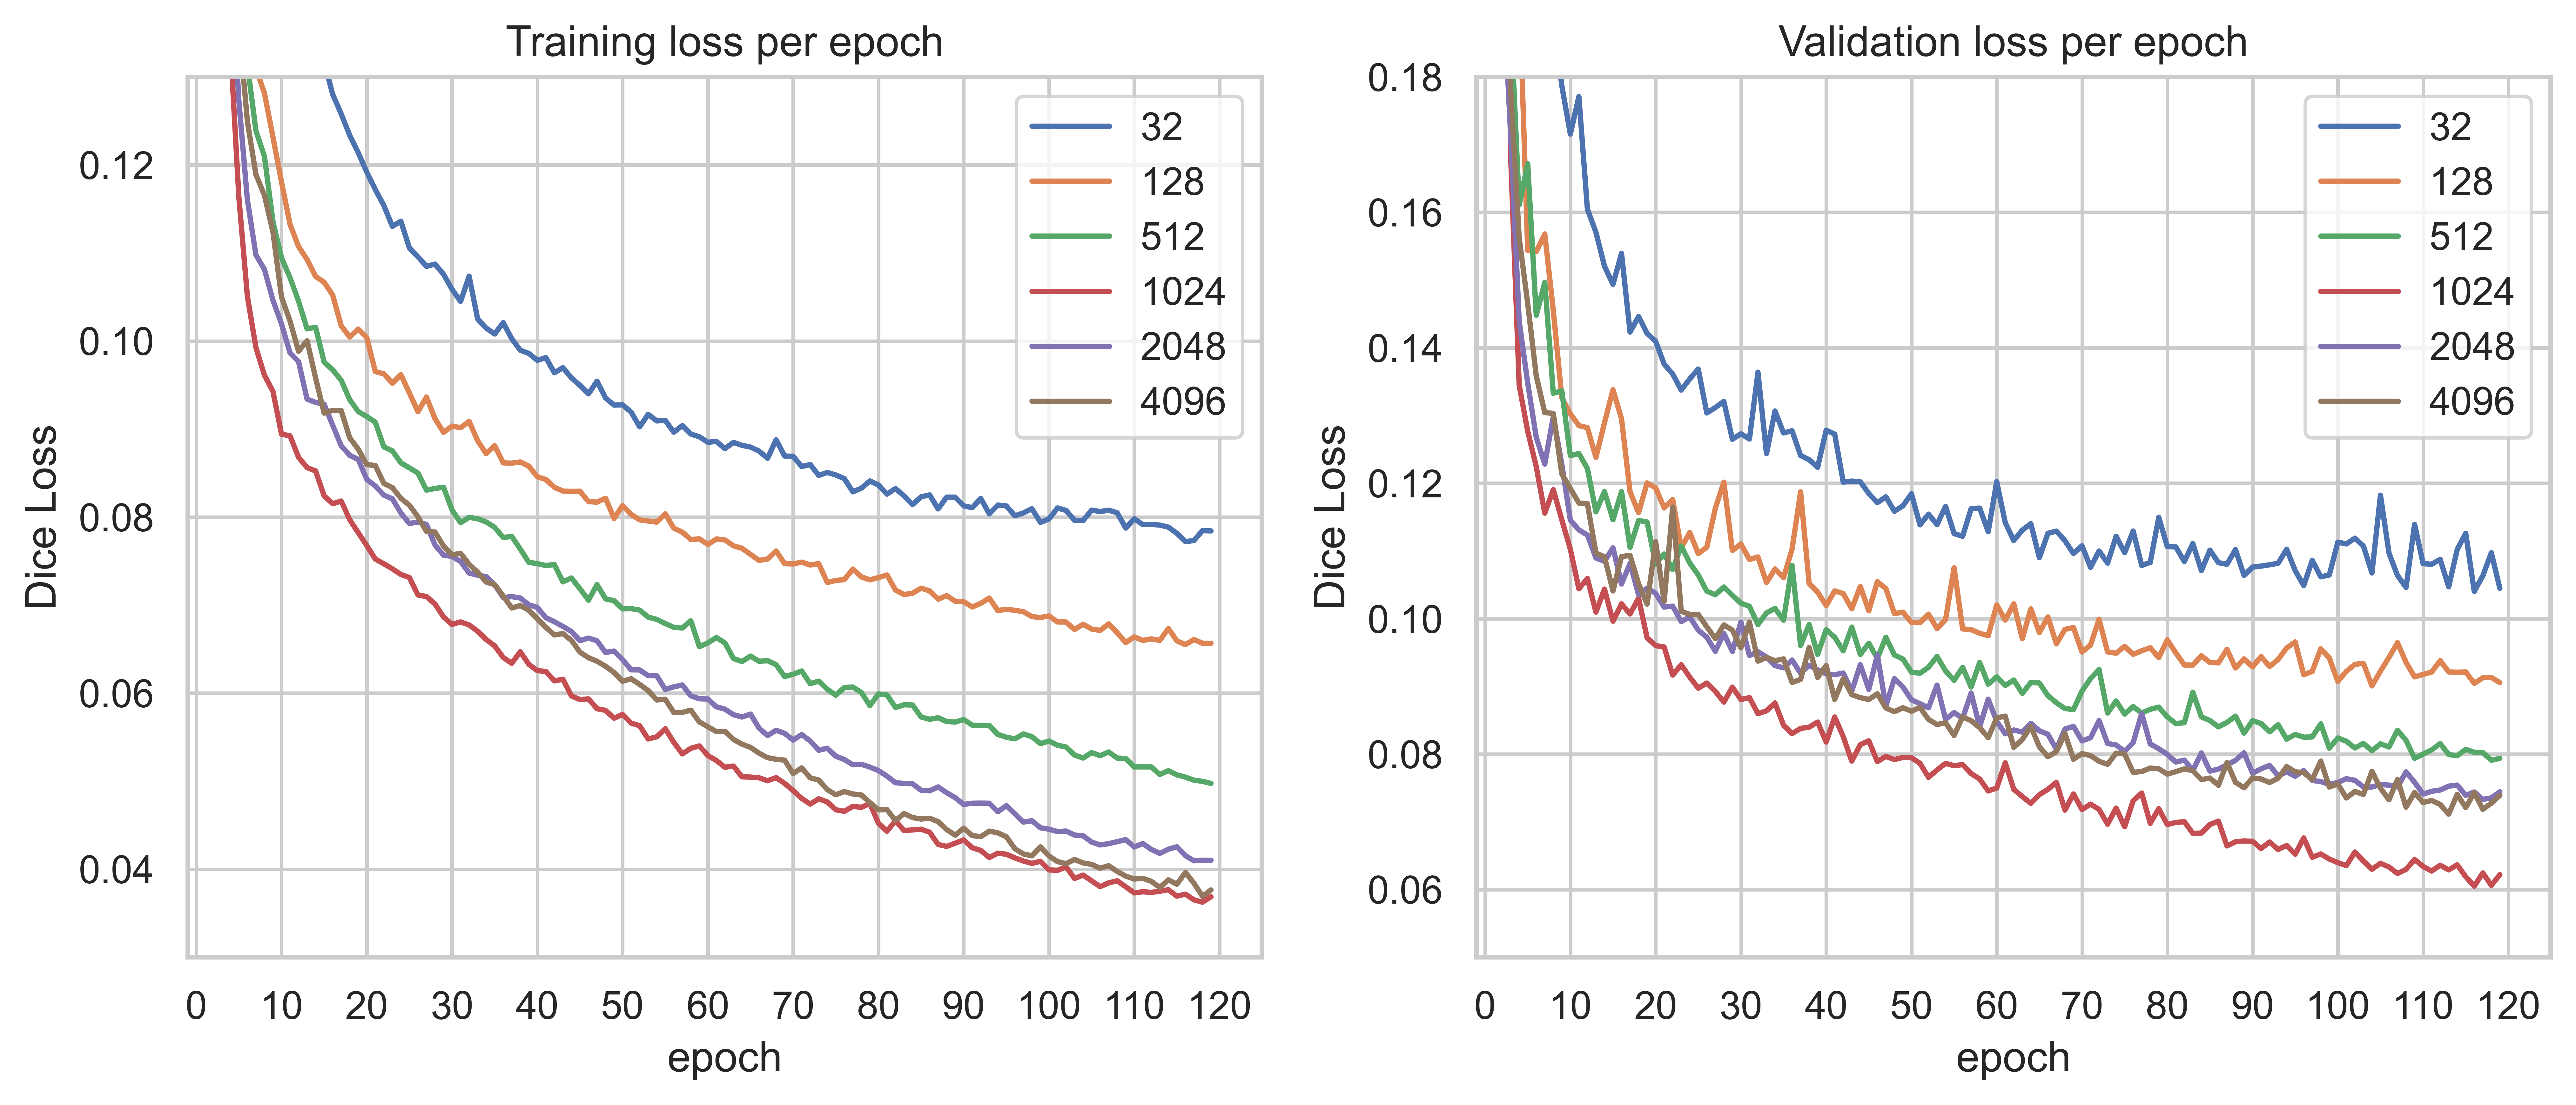
\includegraphics[width=450pt]{figures/ae_latent_space_train_comp}
  \caption{Comparison of average training and validation loss across all batches per epoch for a selection of latent space sizes. The validation loss is calculated at the end of each epoch, hence it can be better than the training loss in certain epochs}\label{latent_space_train_comp}
\end{figure}

For the following evaluation in \autoref{chapter:evaluation} we chose the last epoch that provided the best validation loss and therefore generalization.

All trainings have been executed using the PyTorch framework. The larger networks with a bigger latent space were trained on an NVIDIA Quadro RTX 8000 while the smaller networks were executed on either an NVIDIA Quadro RTX 6000 or an NVIDIA Quadro P5000.



%- short intro, maybe use image, CNN as architecture, DiceLoss, mindim, latentdim, etc. → show final architecture \newline
%- training results: loss, reconstruction example (example maybe in qualitative eval?) \newline
%- alternative network architectures \newline
%\subsection{Regressor Lucas part whatever}

%%%%%%%%%%%%%%%
%%% VAE
%%%%%%%%%%%%%%%
\subsection{Variational Autoencoder}
Trying to further improve the performance of our autoencoders we experimented with Variational autoencoders (VAE). While being simplistic, basic autoencoders have the potential disadvantage of allowing limited control over the latent space. VAEs enforce a distribution over the latent space by penalizing deviations from a previously selected distribution during training, which can produce more continuous and organized latent spaces \todo{find source}. Usually this property is used to generate previously unseen output by randomly sampling from the latent space. However, we investigated if this characteristic is also beneficial for similarity preservation.
\subsubsection{Neural Network}
For comparability and simplicity, the VAE network mostly replicates the autoencoder network from \autoref{autoencoder_network}. The key difference is that the last linear layer before the latent space is replaced by 2 separate linear layers that receive the same input and output the mean $\mu$ and the logarithm of the variance $\log{\sigma^2}$. These values are then used to reparameterize and finally output a latent space vector. The rest of the networks remains unchanged. The adaption is visualized in \autoref{fig_var_autoencoder_network}. Our implementation of the VAE specific parts is similar to the MONAI implementation \parencite{The_MONAI_Consortium2020-ns}, which itself is based on \parencite{Kingma2013}.

\begin{figure}[htbp]
  \centering
  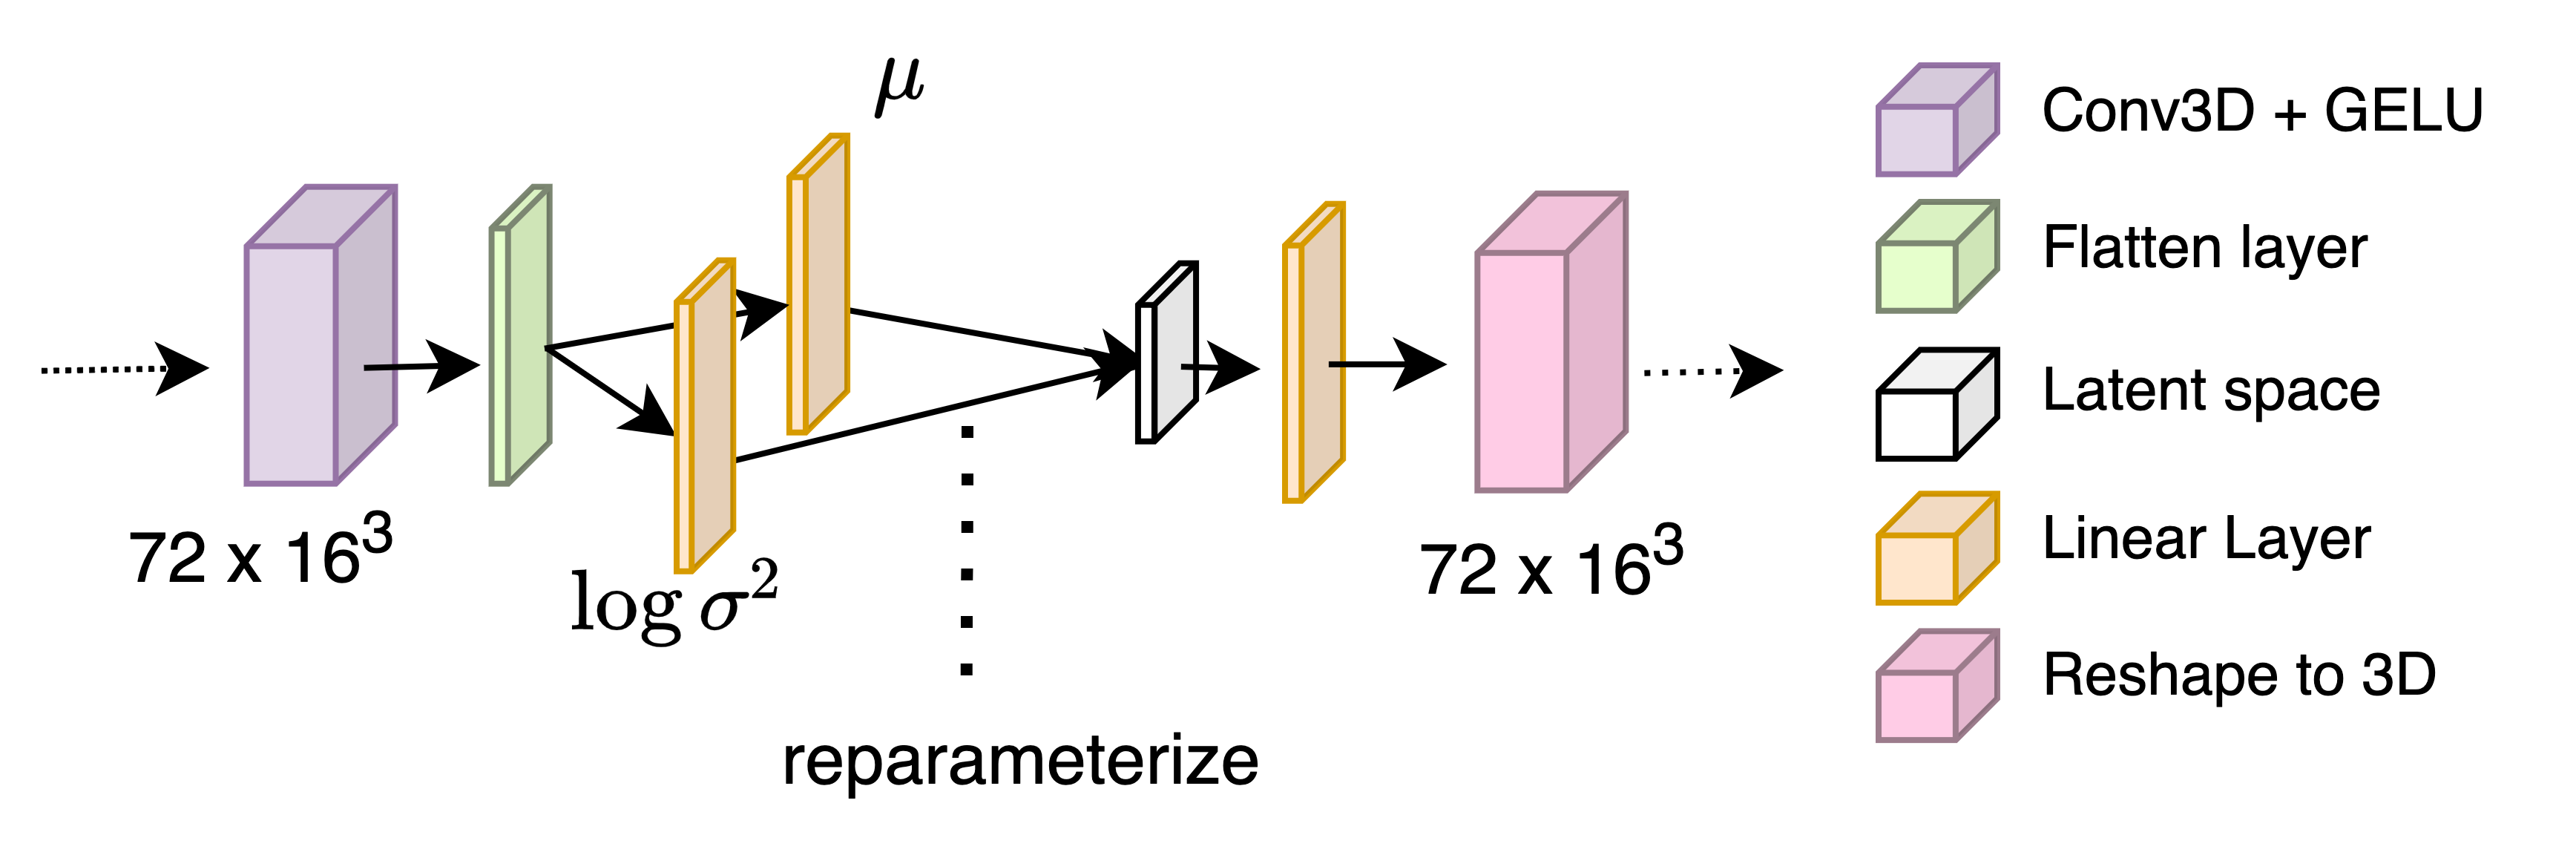
\includegraphics[width=450pt]{figures/var_autoencoder_network}
  \caption{Adaptions to the autoencoder network from \autoref{fig_autoencoder_network}}\label{fig_var_autoencoder_network}
\end{figure}
\FloatBarrier
\subsubsection{Training}
A few aspects, such as training and validation set size, batch size and the optimizer have been reused from \autoref{autoencoder_training}.
Since a VAE also has to consider the latent space distribution during training, the loss function has been adapted to include the Kullback–Leibler divergence $D_{KL}$ (a measure of how similar two distributions are) with a weighting factor of $\beta$ \parencite{betaVAE}. Therefore, the combined loss is calculated as $loss = DiceLoss + \beta * D_{KL}$. 
Basic VAEs use no such weighting factor, and therefore implicitly $\beta = 1$. \parencite{betaVAE} shows that $\beta$ can be used to balance latent channel capacity and independence constraints with reconstruction accuracy. 
Typically, $\beta > 1$ is chosen, however our experiments showed that these common values prevented the network from properly reconstructing the tumor data, leading to a choice of a rather small factor of $\beta = 0.001$.\todo{add better explanation, maybe figure}\\
Note: This small $\beta$ limits the potential of the VAE framework but was necessary to learn an encoding that allowed reconstruction. Moreover, we increased the learning rate to $3e^{-5}$ and reassessed different values for the latent space size.
\autoref{vae_latent_space_train_comp} compares training and validation loss, as well as the $D_{KL}$ and Dice part of the train loss. \todo{epoch, more details about attempts}
Interestingly, our VAE achieves better results with smaller latent sizes, leading to an optimal value of 8, which outperformed the other values in all categories.\\
All trainings have again been executed using the PyTorch framework on either an NVIDIA Quadro RTX 6000 or an NVIDIA Quadro P5000.

\begin{figure}[htbp]
  \centering
  \includegraphics[width=450pt]{figures/vae_latent_space_train_comp}
  \caption{
  Comparison of average training and validation loss across all batches per epoch for a selection of latent space sizes.
  The validation loss is calculated at the end of each epoch, hence it can be better than the training loss.
  The diagrams in the bottom row showcase the dice and $D_{KL}$ part of the training loss.
  \todo{update adn change kld}
  }\label{vae_latent_space_train_comp}
\end{figure}







